\setcounter{framenumber}{-1}
\begin{frame}{Lang(u)age}
\begin{center}
\begin{tikzpicture}
\def\hsep{3}
\def\iw{2}

\def\flagw{2}
\def\flagsep{1.5}

\draw (-\hsep/2,0) node (oral_icon) {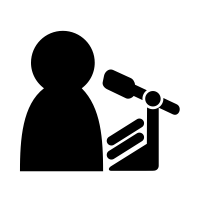
\includegraphics[width=\iw cm]{\PhDthesisdir/plots_and_images/misc_for_slides/oral_icon.png}} ;
\draw (+\hsep/2,0) node (slides_icon) {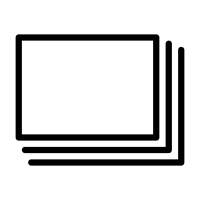
\includegraphics[width=\iw cm]{\PhDthesisdir/plots_and_images/misc_for_slides/slides_icon.png}} ;

\draw (oral_icon.south west) + (-120:\flagsep) node [left] (FR_flag) {
\includegraphics[width=\iw cm]{\PhDthesisdir/plots_and_images/misc_for_slides/flag-france.jpg}} ;
\draw (slides_icon.south east) + (-60:\flagsep) node [right] (EN_flag) {
\includegraphics[width=\iw cm]{\PhDthesisdir/plots_and_images/misc_for_slides/flag-UK.png}} ;

\draw [thick, -latex] (oral_icon.south west) -- (FR_flag.north east);
\draw [thick, -latex] (slides_icon.south east) -- (EN_flag.north west);
\end{tikzpicture}
\end{center}
\end{frame}

\begin{frame}[noframenumbering] \thispagestyle{empty}
\vspace{-.75cm}


\includegraphics[height=1.25cm]{\PhDthesisdir/plots_and_images/logos/ES-R-I_horizontal.pdf}
\hfill

\includegraphics[height=1.25cm]{\PhDthesisdir/plots_and_images/logos/phast-logo.png}
\hfill

\includegraphics[height=1.25cm]{\PhDthesisdir/plots_and_images/logos/Planche_UdL_LogoLyon1Sig_CoulCmjnVecto-eps-converted-to.pdf}

\vfill

\titlepage

\vfill

~ \hfill

\includegraphics[height=1.25cm]{\PhDthesisdir/plots_and_images/logos/IN2P3-B_SignV_bleu-eps-converted-to.pdf}
\hfill

\includegraphics[height=1.25cm]{\PhDthesisdir/plots_and_images/logos/CERN-logo.jpg}
\hfill
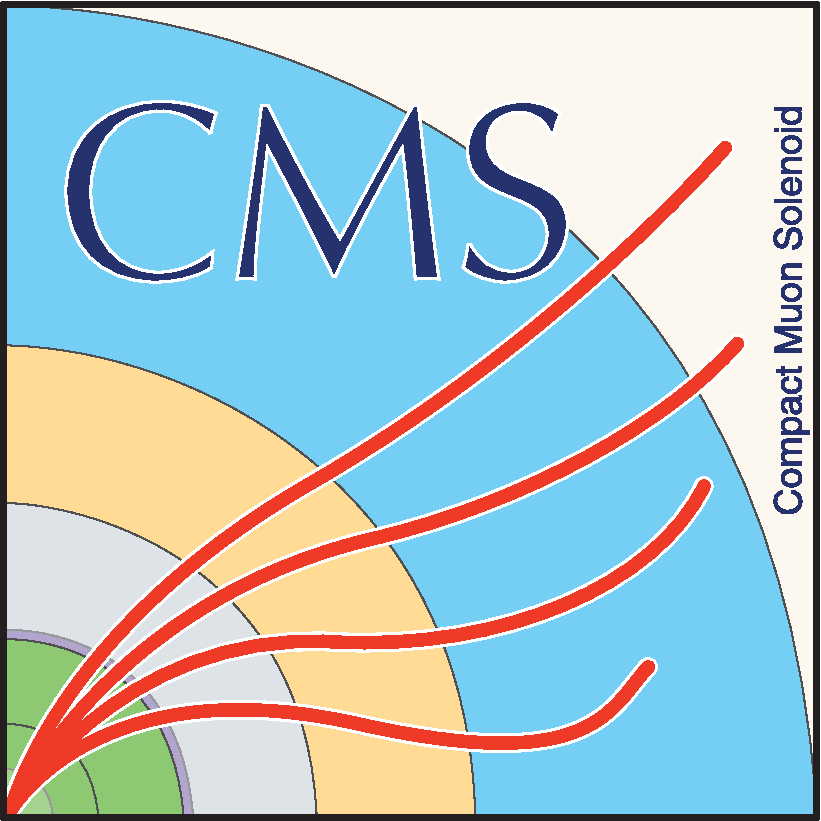
\includegraphics[height=1.25cm]{\PhDthesisdir/plots_and_images/logos/CMS_logo.pdf}
\hfill

\includegraphics[height=1.25cm]{\PhDthesisdir/plots_and_images/logos/logo_IP2I.jpg}
\hfill ~

\vspace{-.5cm}
\end{frame}

\begin{frame}

\begin{center}
Why do we \textbf{search for...}?
\end{center}

\begin{minipage}[c]{.45\textwidth}
\begin{block}{Current model status}
\begin{itemize}
\item Robust and predictive (top quark, \Wboson, \Zboson\ and one Higgs boson...)
\item still not good enough, unable to explain some observations such as:
\begin{itemize}
\item dark matter $\longrightarrow$
\item matter vs antimatter asymmetry
\item ...
\end{itemize}
\item Go beyond with a new model!
\item Consequences of this new model? \textbf{\color{ltcolorred}Test it!}
\end{itemize}
\end{block}
\end{minipage}
\hfill
\begin{minipage}[c]{.45\textwidth}
\begin{center}
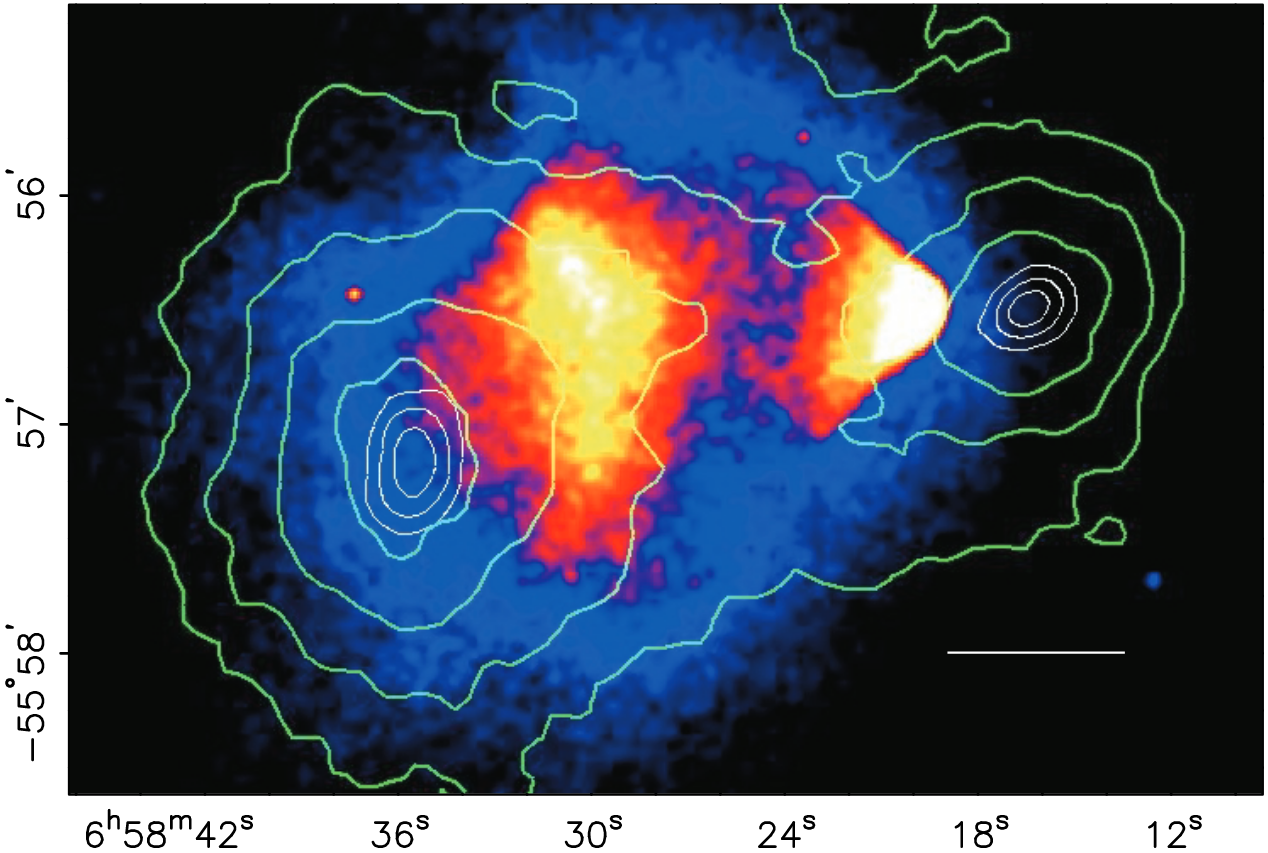
\includegraphics[width=.9\linewidth]{\PhDthesisdir/plots_and_images/from_Clowe_2006/bullet_cluster.png}
\end{center}
\end{minipage}
\beamercite{Clowe_2006}
\end{frame}

\begin{frame}{Keywords in title}
\begin{center}
\small
\begin{tikzpicture}
\draw (0,0) node [below right] (t1) {Search for\vphantom{Àq}};
\draw (t1.east) node (t2) [right] {\color{ltcolorcyan}\textbf{additional}\vphantom{Àq}};
\draw (t2.east) node (t3) [right] {\color{ltcolormagenta}\textbf{neutral}\vphantom{Àq}};
\draw (t3.east) node (t4) [right] {\color{ltcolorgreen}\textbf{Higgs bosons}\vphantom{Àq}};
\draw (t4.east) node (t5) [right] {\color{ltcolororange}\textbf{decaying to tau lepton pair}\vphantom{Àq}};
\draw (t5.east) node (t6) [right] {in the\vphantom{Àq}};
\draw (t6.east) node (t7) [right] {\color{ltcolorred}\textbf{CMS experiment}\vphantom{Àq}};
\draw (t7.east) node (t8) [right] {at\vphantom{Àq}};
\draw (t8.east) node (t9) [right] {\color{ltcolorblue}\textbf{LHC}\vphantom{Àq}};

%\draw [thick, -latex] (t4.south) --+ (0,-.5) node (l1) [below] {type of particle};
%\draw [thick, -latex] (l1.south) --+ (0,-.5) node (l2) [below] {why this one?};
%
%\draw [thick, -latex] (t3.south) --+ (-.75,-1) node (l4) [below] {no electric charge};
%\draw [thick, -latex] (l4.south) --+ (0,-.5) node (l5) [below] {means some have?};
%
%\draw [thick, -latex] (t2.south) --+ (-1.25,-1.5) node (l6) [below] {already one!};
%
%\draw [thick, -latex] (l5.south) --+ (0,-1) node (l3) [below] {Part~I\vphantom{Àq}};
%\draw [thick, -latex] (l2.south) -- (l3);
%\draw [thick, -latex] (l6.south) -- (l3);
%\draw  (l3.south) node (l3bis) {\emph{Phenomenology}};
%
%\draw  [thick, -latex] (t9.south) --+ (0,-.5) node (l8) [below] {gives "something"};
%\draw  (l8.south) node (l9) {to measure};
%
%\draw  [thick, -latex] (t7.south) --+ (0,-1.5) node (l7) [below] {measurements};
%\draw [thick, dashed, -latex] (l9.south) -- (l7.east);
%
%\draw (l7.east) + (0,-1.5) node (l10) [below] {Part~II\vphantom{Àq}};
%\draw [thick, -latex] (l9.south) -- (l10);
%\draw [thick, -latex] (l7.south) -- (l10);
%\draw  (l10.south) node (l10bis) {\emph{Experimental device}};
%
%\draw [thick, -latex] (t5.south) --+ (0,-1.25) node (l11) [below] {why this case?};
%\draw [thick, -latex] (l11.south west) -- (l3);
%\draw [thick, -latex] (l11.south) --+ (0,-.5) node (l13) [below] {results?};
%\draw [thick, -latex] (l13.south) --+ (0,-.75) node (l12) [below] {Part~III\vphantom{Àq}};
%\draw  (l12.south) node (l12bis) {\emph{$\Higgs\to\tau\tau$ analysis}};
%
%\draw (\textwidth/2,-.725\textheight) node [above] {+ Part~IV: \emph{Machine Learning use in the $\Higgs\to\tau\tau$ analysis}};
\draw (.99\textwidth,-.725\textheight) coordinate (a);
\end{tikzpicture}
\end{center}
\end{frame}
\addtocounter{framenumber}{-1}
\begin{frame}{Keywords in title}
\begin{center}
\small
\begin{tikzpicture}
\draw (0,0) node [below right] (t1) {Search for\vphantom{Àq}};
\draw (t1.east) node (t2) [right] {\color{ltcolorcyan}\textbf{additional}\vphantom{Àq}};
\draw (t2.east) node (t3) [right] {\color{ltcolormagenta}\textbf{neutral}\vphantom{Àq}};
\draw (t3.east) node (t4) [right] {\color{ltcolorgreen}\textbf{Higgs bosons}\vphantom{Àq}};
\draw (t4.east) node (t5) [right] {\color{ltcolororange}\textbf{decaying to tau lepton pair}\vphantom{Àq}};
\draw (t5.east) node (t6) [right] {in the\vphantom{Àq}};
\draw (t6.east) node (t7) [right] {\color{ltcolorred}\textbf{CMS experiment}\vphantom{Àq}};
\draw (t7.east) node (t8) [right] {at\vphantom{Àq}};
\draw (t8.east) node (t9) [right] {\color{ltcolorblue}\textbf{LHC}\vphantom{Àq}};

\draw [thick, -latex] (t4.south) --+ (0,-.5) node (l1) [below] {type of particle};
\draw [thick, -latex] (l1.south) --+ (0,-.5) node (l2) [below] {why this one?};

\draw [thick, -latex] (t3.south) --+ (-.75,-1) node (l4) [below] {no electric charge};
\draw [thick, -latex] (l4.south) --+ (0,-.5) node (l5) [below] {means some have?};

\draw [thick, -latex] (t2.south) --+ (-1.25,-1.5) node (l6) [below] {already one!};

\draw [thick, -latex] (l5.south) --+ (0,-1) node (l3) [below] {Part~I\vphantom{Àq}};
\draw [thick, -latex] (l2.south) -- (l3);
\draw [thick, -latex] (l6.south) -- (l3);
\draw  (l3.south) node (l3bis) {\emph{Phenomenology}};

%\draw  [thick, -latex] (t9.south) --+ (0,-.5) node (l8) [below] {gives "something"};
%\draw  (l8.south) node (l9) {to measure};
%
%\draw  [thick, -latex] (t7.south) --+ (0,-1.5) node (l7) [below] {measurements};
%\draw [thick, dashed, -latex] (l9.south) -- (l7.east);
%
%\draw (l7.east) + (0,-1.5) node (l10) [below] {Part~II\vphantom{Àq}};
%\draw [thick, -latex] (l9.south) -- (l10);
%\draw [thick, -latex] (l7.south) -- (l10);
%\draw  (l10.south) node (l10bis) {\emph{Experimental device}};
%
\draw [thick, -latex] (t5.south) --+ (0,-1.25) node (l11) [below] {why this case?};
\draw [thick, -latex] (l11.south west) -- (l3);
%\draw [thick, -latex] (l11.south) --+ (0,-.5) node (l13) [below] {results?};
%\draw [thick, -latex] (l13.south) --+ (0,-.75) node (l12) [below] {Part~III\vphantom{Àq}};
%\draw  (l12.south) node (l12bis) {\emph{$\Higgs\to\tau\tau$ analysis}};
%
%\draw (\textwidth/2,-.725\textheight) node [above] {+ Part~IV: \emph{Machine Learning use in the $\Higgs\to\tau\tau$ analysis}};
\draw (.99\textwidth,-.725\textheight) coordinate (a);
\end{tikzpicture}
\end{center}
\end{frame}
\addtocounter{framenumber}{-1}
\begin{frame}{Keywords in title}
\begin{center}
\small
\begin{tikzpicture}
\draw (0,0) node [below right] (t1) {Search for\vphantom{Àq}};
\draw (t1.east) node (t2) [right] {\color{ltcolorcyan}\textbf{additional}\vphantom{Àq}};
\draw (t2.east) node (t3) [right] {\color{ltcolormagenta}\textbf{neutral}\vphantom{Àq}};
\draw (t3.east) node (t4) [right] {\color{ltcolorgreen}\textbf{Higgs bosons}\vphantom{Àq}};
\draw (t4.east) node (t5) [right] {\color{ltcolororange}\textbf{decaying to tau lepton pair}\vphantom{Àq}};
\draw (t5.east) node (t6) [right] {in the\vphantom{Àq}};
\draw (t6.east) node (t7) [right] {\color{ltcolorred}\textbf{CMS experiment}\vphantom{Àq}};
\draw (t7.east) node (t8) [right] {at\vphantom{Àq}};
\draw (t8.east) node (t9) [right] {\color{ltcolorblue}\textbf{LHC}\vphantom{Àq}};

\draw [thick, -latex] (t4.south) --+ (0,-.5) node (l1) [below] {type of particle};
\draw [thick, -latex] (l1.south) --+ (0,-.5) node (l2) [below] {why this one?};

\draw [thick, -latex] (t3.south) --+ (-.75,-1) node (l4) [below] {no electric charge};
\draw [thick, -latex] (l4.south) --+ (0,-.5) node (l5) [below] {means some have?};

\draw [thick, -latex] (t2.south) --+ (-1.25,-1.5) node (l6) [below] {already one!};

\draw [thick, -latex] (l5.south) --+ (0,-1) node (l3) [below] {Part~I\vphantom{Àq}};
\draw [thick, -latex] (l2.south) -- (l3);
\draw [thick, -latex] (l6.south) -- (l3);
\draw  (l3.south) node (l3bis) {\emph{Phenomenology}};

\draw  [thick, -latex] (t9.south) --+ (0,-.5) node (l8) [below] {gives "something"};
\draw  (l8.south) node (l9) {to measure};

\draw  [thick, -latex] (t7.south) --+ (0,-1.5) node (l7) [below] {measurements};
\draw [thick, dashed, -latex] (l9.south) -- (l7.east);

\draw (l7.east) + (0,-1.5) node (l10) [below] {Part~II\vphantom{Àq}};
\draw [thick, -latex] (l9.south) -- (l10);
\draw [thick, -latex] (l7.south) -- (l10);
\draw  (l10.south) node (l10bis) {\emph{Experimental device}};
%
\draw [thick, -latex] (t5.south) --+ (0,-1.25) node (l11) [below] {why this case?};
\draw [thick, -latex] (l11.south west) -- (l3);
%\draw [thick, -latex] (l11.south) --+ (0,-.5) node (l13) [below] {results?};
%\draw [thick, -latex] (l13.south) --+ (0,-.75) node (l12) [below] {Part~III\vphantom{Àq}};
%\draw  (l12.south) node (l12bis) {\emph{$\Higgs\to\tau\tau$ analysis}};
%
%\draw (\textwidth/2,-.725\textheight) node [above] {+ Part~IV: \emph{Machine Learning use in the $\Higgs\to\tau\tau$ analysis}};
\draw (.99\textwidth,-.725\textheight) coordinate (a);
\end{tikzpicture}
\end{center}
\end{frame}
\addtocounter{framenumber}{-1}
\begin{frame}{Keywords in title}
\begin{center}
\small
\begin{tikzpicture}
\draw (0,0) node [below right] (t1) {Search for\vphantom{Àq}};
\draw (t1.east) node (t2) [right] {\color{ltcolorcyan}\textbf{additional}\vphantom{Àq}};
\draw (t2.east) node (t3) [right] {\color{ltcolormagenta}\textbf{neutral}\vphantom{Àq}};
\draw (t3.east) node (t4) [right] {\color{ltcolorgreen}\textbf{Higgs bosons}\vphantom{Àq}};
\draw (t4.east) node (t5) [right] {\color{ltcolororange}\textbf{decaying to tau lepton pair}\vphantom{Àq}};
\draw (t5.east) node (t6) [right] {in the\vphantom{Àq}};
\draw (t6.east) node (t7) [right] {\color{ltcolorred}\textbf{CMS experiment}\vphantom{Àq}};
\draw (t7.east) node (t8) [right] {at\vphantom{Àq}};
\draw (t8.east) node (t9) [right] {\color{ltcolorblue}\textbf{LHC}\vphantom{Àq}};

\draw [thick, -latex] (t4.south) --+ (0,-.5) node (l1) [below] {type of particle};
\draw [thick, -latex] (l1.south) --+ (0,-.5) node (l2) [below] {why this one?};

\draw [thick, -latex] (t3.south) --+ (-.75,-1) node (l4) [below] {no electric charge};
\draw [thick, -latex] (l4.south) --+ (0,-.5) node (l5) [below] {means some have?};

\draw [thick, -latex] (t2.south) --+ (-1.25,-1.5) node (l6) [below] {already one!};

\draw [thick, -latex] (l5.south) --+ (0,-1) node (l3) [below] {Part~I\vphantom{Àq}};
\draw [thick, -latex] (l2.south) -- (l3);
\draw [thick, -latex] (l6.south) -- (l3);
\draw  (l3.south) node (l3bis) {\emph{Phenomenology}};

\draw  [thick, -latex] (t9.south) --+ (0,-.5) node (l8) [below] {gives "something"};
\draw  (l8.south) node (l9) {to measure};

\draw  [thick, -latex] (t7.south) --+ (0,-1.5) node (l7) [below] {measurements};
\draw [thick, dashed, -latex] (l9.south) -- (l7.east);

\draw (l7.east) + (0,-1.5) node (l10) [below] {Part~II\vphantom{Àq}};
\draw [thick, -latex] (l9.south) -- (l10);
\draw [thick, -latex] (l7.south) -- (l10);
\draw  (l10.south) node (l10bis) {\emph{Experimental device}};

\draw [thick, -latex] (t5.south) --+ (0,-1.25) node (l11) [below] {why this case?};
\draw [thick, -latex] (l11.south west) -- (l3);
\draw [thick, -latex] (l11.south) --+ (0,-.5) node (l13) [below] {results?};
\draw [thick, -latex] (l13.south) --+ (0,-.75) node (l12) [below] {Part~III\vphantom{Àq}};
\draw  (l12.south) node (l12bis) {\emph{$\Higgs\to\tau\tau$ analysis}};

%\draw (\textwidth/2,-.725\textheight) node [above] {+ Part~IV: \emph{Machine Learning use in the $\Higgs\to\tau\tau$ analysis}};
\draw (.99\textwidth,-.725\textheight) coordinate (a);
\end{tikzpicture}
\end{center}
\end{frame}
\addtocounter{framenumber}{-1}
\begin{frame}{Keywords in title}
\begin{center}
\small
\begin{tikzpicture}
\draw (0,0) node [below right] (t1) {Search for\vphantom{Àq}};
\draw (t1.east) node (t2) [right] {\color{ltcolorcyan}\textbf{additional}\vphantom{Àq}};
\draw (t2.east) node (t3) [right] {\color{ltcolormagenta}\textbf{neutral}\vphantom{Àq}};
\draw (t3.east) node (t4) [right] {\color{ltcolorgreen}\textbf{Higgs bosons}\vphantom{Àq}};
\draw (t4.east) node (t5) [right] {\color{ltcolororange}\textbf{decaying to tau lepton pair}\vphantom{Àq}};
\draw (t5.east) node (t6) [right] {in the\vphantom{Àq}};
\draw (t6.east) node (t7) [right] {\color{ltcolorred}\textbf{CMS experiment}\vphantom{Àq}};
\draw (t7.east) node (t8) [right] {at\vphantom{Àq}};
\draw (t8.east) node (t9) [right] {\color{ltcolorblue}\textbf{LHC}\vphantom{Àq}};

\draw [thick, -latex] (t4.south) --+ (0,-.5) node (l1) [below] {type of particle};
\draw [thick, -latex] (l1.south) --+ (0,-.5) node (l2) [below] {why this one?};

\draw [thick, -latex] (t3.south) --+ (-.75,-1) node (l4) [below] {no electric charge};
\draw [thick, -latex] (l4.south) --+ (0,-.5) node (l5) [below] {means some have?};

\draw [thick, -latex] (t2.south) --+ (-1.25,-1.5) node (l6) [below] {already one!};

\draw [thick, -latex] (l5.south) --+ (0,-1) node (l3) [below] {Part~I\vphantom{Àq}};
\draw [thick, -latex] (l2.south) -- (l3);
\draw [thick, -latex] (l6.south) -- (l3);
\draw  (l3.south) node (l3bis) {\emph{Phenomenology}};

\draw  [thick, -latex] (t9.south) --+ (0,-.5) node (l8) [below] {gives "something"};
\draw  (l8.south) node (l9) {to measure};

\draw  [thick, -latex] (t7.south) --+ (0,-1.5) node (l7) [below] {measurements};
\draw [thick, dashed, -latex] (l9.south) -- (l7.east);

\draw (l7.east) + (0,-1.5) node (l10) [below] {Part~II\vphantom{Àq}};
\draw [thick, -latex] (l9.south) -- (l10);
\draw [thick, -latex] (l7.south) -- (l10);
\draw  (l10.south) node (l10bis) {\emph{Experimental device}};

\draw [thick, -latex] (t5.south) --+ (0,-1.25) node (l11) [below] {why this case?};
\draw [thick, -latex] (l11.south west) -- (l3);
\draw [thick, -latex] (l11.south) --+ (0,-.5) node (l13) [below] {results?};
\draw [thick, -latex] (l13.south) --+ (0,-.75) node (l12) [below] {Part~III\vphantom{Àq}};
\draw  (l12.south) node (l12bis) {\emph{$\Higgs\to\tau\tau$ analysis}};

\draw (\textwidth/2,-.725\textheight) node [above] {+ Part~IV: \emph{Machine Learning use in the $\Higgs\to\tau\tau$ analysis}};
\draw (.99\textwidth,-.725\textheight) coordinate (a);
\end{tikzpicture}
\end{center}
\end{frame}